\chapter{Compensating \acs{erp} jitter for gaze-independence}%
\label{sec:covert-align}
\epigraph{``You see, but you do not observe!''}{Sherlock Holmes in  \\ \emph{A
Scandal in Bohemia -- Sir Arthur Conan Doyle}}
\noindent\emph{This chapter was published as part of~\textcite{VanDenKerchove2024}.}

\section{Introduction}

The decoding methods described in \cref{sec:stbf-struct} and
\cref{sec:bttda} are general attempts at increasing \ac{erp} decoding accuracy.
Given the problem statement of this work, we are also interested in targeted
methods that would specifically advance the development of gaze-independent
visual \acp{bci} (see \cref{sec:gaze-independence/sota}).
Methods of directly enhancing gaze-independent decoding through optimizing
decoder design have not been widely studied (see
\cref{sec:gaze-independence/sota/decoding}).
We assume that advances in gaze-independent decoding can be made if properties
of covert \ac{vsa} that affect performance can be identified and accounted for.
The latency estimation and alignment approach proposed in \cref{sec:wcble}
was specifically designed for this purpose.

\textcite{Arico2014} observed higher variability in single-trial P3 peak
latencies relative to stimulus onset during covert \ac{vsa} (529 ms$^2$) compared to overt
\ac{vsa} (256$^2$ ms).
This latency variability contributes to reduced covert \ac{vsa} decoding performance.
While they proposed an analysis and performance prediction method, they did not provide a
decoding solution.
They suggested that compensating for latency jitter could enhance covert \ac{vsa}
decoding, but did not verify this hypothesis directly.
Additionally, \textcite{Hardiansyah2020} developed a classifier for
covert \ac{vsa} \acp{erp}, exploiting single-trial latency features in combination with
amplitude features for classification with a support vector machine.
They demonstrated the positive influence of single-trial \ac{erp} component latency
features on covert \ac{vsa} inference, yet did not attempt to correct the amplitude
features for these latencies.

Furthermore, as mentioned in \cref{sec:gaze-independence/sota/visual} and
\cref{sec:gaze-independence/approach/cvsa-erp},
our goal is also to explore more flexible gaze-independent settings than the
usual covert \ac{vsa} with central gaze fixation reported in most literature.
\textcite{Frenzel2011} introduced a similar protocol to the proposed split
\ac{vsa} setting (see~\cref{fig:gaze/vsa/free}).
They showed that it is possible to perform split \ac{vsa} and that, in this
case, visuospatial attention and gaze direction can be decoded separately using
classical \ac{erp} techniques.
To the best of our
knowledge, this is the sole study that investigated split attention in \ac{erp}-based \acp{bci}.
However, \textcite{Frenzel2011} considered their interface only for the case
where the user actively intends to select both targets determined by the gaze
and the \ac{vsa}.
In the split \ac{vsa} setting considered in our work, we instruct the participant to ignore
the distractor and only attend to the cued target, as we are interested in
decoding the visuospatial attention only.

\section{Materials \& methods}

\subsection{Data collection}
We evaluate our approach on a dataset specifically recorded for this study, designed to
probe different modalities of covert \ac{vsa}, and on the publicly available
BNCI2014-009 dataset~\cite{Aloise2012a}.

\subsubsection{CVSA-ERP dataset}%
\label{sec:covert-align/stimulation}

We recorded a dataset to validate our approach.
The Covert Visuospatial Attention \ac{erp} (CVSA-ERP) dataset
consists of 15 participants, mean age $26.34\pm3.04$ years.
This study was approved by the Ethics Commission of University Hospital Leuven
(S62547).
Each subject performed different \ac{vsa} conditions (overt, covert, and split),
illustrated in Figure~\ref{fig:interface} (top row).
Using a hexagonal layout interface, similar to the visual Hex-o-Spell proposed
by \textcite{Treder2010}, we presented six flashing targets (without letters or
symbols) to the participant while the \ac{eeg}, electrooculogram (EOG), and the
participant's eye gaze using eye tracking were recorded.
The \ac{vsa} conditions described in the first row of Figure~\ref{fig:interface} are
considered.
\begin{figure*}
  \bigskip
	\begin{subfigure}{\linewidth}
		\caption{}%
		\label{fig:interface}
		\includegraphics[width=\linewidth]{figures/covert_align/figure3a.pdf}
	\end{subfigure}

	\bigskip
	\bigskip
	\begin{subfigure}{\linewidth}
		\caption{}%
		\label{fig:erps}
		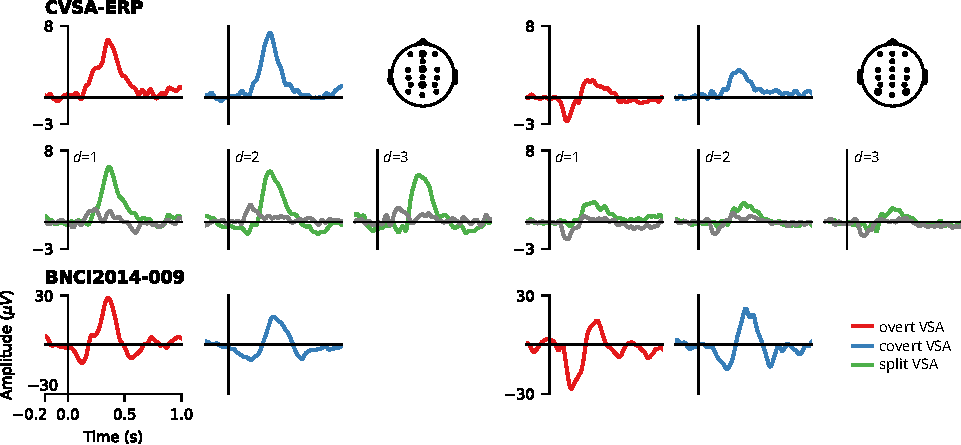
\includegraphics[width=\linewidth]{figures/covert_align/figure3b.pdf}
	\end{subfigure}%

  \caption[Stimulation interfaces and evoked \acsp{erp}.]{%
		\subref{fig:interface} Interfaces and visuospatial attention (\ac{vsa})
    conditions in the CVSA-ERP and BNCI2014-009 datasets.
		In the CVSA-ERP oddball \ac{bci} interface, screen targets are intensified one after
    the other in pseudorandom order while the participant can either pay overt,
    covert, or split \ac{vsa} to the cued target.
		In the BNCI2014-009 overt \ac{vsa} interface, entire rows and columns are
		intensified at once. In its covert counterpart,
		groups of 6 letters are intensified one after the other, partly relying on
    feature attention.
		\subref{fig:erps} Contrast between target (color) and non-target, and
    distractor (gray) and non-target grand average event-related potentials per \ac{vsa} condition and dataset.
    Overt \ac{vsa} yields a strong modulation of the N1 component in both datasets;
    the P3 amplitude decreases with the degree of split \ac{vsa}.
    In split \ac{vsa}, N1 and P2 are more prominently evoked by the distractor,
    while the P3 is evoked by the target.
	}
\end{figure*}

In contrast to the protocol proposed by \textcite{Frenzel2011}, split \ac{vsa} was
performed by instructing the participant to attend to the intensifications of the
cued target and ignore the intensifications of the distractor target.
Since we assume there will be an effect depending on the distance between
the attended target and the distractor, we discern three split \ac{vsa} sub-conditions:
the distractor is either clockwise or counterclockwise directly next to the
attended target ($d=1$), there is one other target between the attended target and
the distractor ($d=2$), or the distractor is opposite the intended target
($d=3$).

\ac{eeg} for the CVSA-ERP dataset was recorded using a SynAmps RT amplifier
(Compumedics Neuroscan, Australia) at 2048 Hz and 62 Ag/AgCl active electrodes arranged in the
international 10-10 layout fitted to a standard electrode cap (EASYCAP GmbH,
Germany), with electrodes located at AFz and FCz as ground and reference, respectively.
Using electrolyte gel, electrode impedances were brought below 5k$\Omega$.
Electrodes TP9 and TP10, used for off-line re-referencing, were directly
attached to the skin using stickers for better contact.
The power line frequency in Belgium is 50 Hz.
The participant's eye gaze was registered using an EyeLink 1000 Plus eye tracker (SR Research,
Canada) in non-fixation mode.

Participants signed an informed consent form and were seated at a distance of
60 cm from a CRT-emulating monitor (VPixx
Technologies, Canada) operating at a refresh rate of 120 Hz, displaying 6
circular white targets with a diameter of 4.15° visual angle and laid out on a hexagon
with a radius of 12.28° of visual angle centered on the midpoint of the screen,
conforming to the interface proposed by \textcite{Treder2010}
(\cref{fig:covert-align/interface/interface}).
A hexagonal layout interface with an empty center and a low number of targets
counteracts target crowding, and as long as the subject’s gaze is within the hexagon of
targets, no other target can be between the subject’s gaze and a covertly
attended target.
Targets are full-contrast white and were intensified by scaling them to a
larger size (5.60° of visual angle, see \cref{fig:covert-align/interface/intensification})
instead of changing the contrast to avoid Troxler-fading\footnote{The optical illusion of disappearing unchanging stimuli
experienced when visually fixating~\cite{Troxler1804}.}~\cite{Treder2010} in the
peripheral visual field.
Stimuli were presented using PsychoPy (version 2023.1.3)~\cite{Peirce2019}.

\begin{figure}
  \begin{subfigure}[t]{.45\textwidth}
    \begin{tikzpicture}[
    scale=\textwidth/5cm
]
% Rectangle background
\fill[muteblack] (-2.5,-2) rectangle (2.5,2);

% Hexagon vertices (white circles)
  \fill[white] (1,0) circle (.35);    % Right
  \fill[white] (-1,0) circle (.35);   % Left
\fill[white] (0.5,0.866) circle (.35); % Top-right
\fill[white] (-0.5,0.866) circle (.35); % Top-left
\fill[white] (0.5,-0.866) circle (.35); % Bottom-right
\fill[white] (-0.5,-0.866) circle (.35); % Bottom-left

\end{tikzpicture}

    \caption[The stimulation interface.]{The stimulation interface based on the visual Hex-o-Spell
    \acs{bci}~\cite{Treder2010}.}%
    \label{fig:covert-align/interface/interface}
  \end{subfigure}\hfill%
  \begin{subfigure}[t]{.45\textwidth}
    \begin{tikzpicture}[
    scale=\textwidth/5cm
]
% Rectangle background
\fill[muteblack] (-2.5,-2) rectangle (2.5,2);

% Hexagon vertices (white circles)
\fill[white] (1,0) circle (.35);    % Right
\fill[white] (-1,0) circle (.35);   % Left
\fill[white] (0.5,0.866) circle (.35); % Top-right
\fill[white] (-0.5,0.866) circle (.45); % Top-left
\fill[white] (0.5,-0.866) circle (.35); % Bottom-right
\fill[white] (-0.5,-0.866) circle (.35); % Bottom-left

\end{tikzpicture}%

    \caption[Intensification.]{When a target is intensified, it is enlarged for
    a very short time.}%
    \label{fig:covert-align/interface/intensification}
  \end{subfigure}

  \begin{subfigure}[t]{.45\textwidth}
    \begin{tikzpicture}[
    scale=\textwidth/5cm
]
% Rectangle background
\fill[muteblack] (-2.5,-2) rectangle (2.5,2);

% Hexagon vertices (white circles)
\fill[white] (1,0) circle (.35);    % Right
\fill[white] (-1,0) circle (.35);   % Left
\fill[white] (0.5,0.866) circle (.35); % Top-right
\fill[white] (-0.5,0.866) circle (.35); % Top-left
\fill[white] (0.5,-0.866) circle (.35); % Bottom-right
\fill[white] (-0.5,-0.866) circle (.35); % Bottom-left
\draw[accent2, ultra thick] (0.9,0) -- (1.1,0);  % Shorter horizontal line
\draw[accent2, ultra thick] (1,-0.1) -- (1,0.1); % Shorter vertical line
\end{tikzpicture}%

    \caption[Gaze fixated on a target.]{In the overt and split \ac{vsa}
    settings, the
    participant is cued to fixate on one of the targets.}%
    \label{fig:covert-align/interface/overt}
  \end{subfigure}\hfill%
  \begin{subfigure}[t]{.45\textwidth}
    \begin{tikzpicture}[
    scale=\textwidth/5cm
]
% Rectangle background
\fill[muteblack] (-2.5,-2) rectangle (2.5,2);

% Hexagon vertices (white circles)
\fill[white] (1,0) circle (.35);    % Right
\fill[white] (-1,0) circle (.35);   % Left
\fill[white] (0.5,0.866) circle (.35); % Top-right
\fill[white] (-0.5,0.866) circle (.35); % Top-left
\fill[white] (0.5,-0.866) circle (.35); % Bottom-right
\fill[white] (-0.5,-0.866) circle (.35); % Bottom-left

% Plus symbol made of two shorter lines at the center (0,0)
\draw[accent2, ultra thick] (-0.1,0) -- (0.1,0);  % Shorter horizontal line
\draw[accent2, ultra thick] (0,-0.1) -- (0,0.1);  % Shorter vertical line
\end{tikzpicture}%

    \caption[Gaze fixated centrally.]{In the covert \ac{vsa} setting, the participant is
    cued to fixate at the center of the interface.}%
    \label{fig:covert-align/interface/covert}
  \end{subfigure}
  \caption[Stimulation interface layout.]{Layout and visual elements of the experimental stimulation
  interface used in recording the CVSA-ERP dataset.}
\end{figure}

The participant was instructed to press the space bar when ready for a block
of stimulations.
Then, one target was indicated as the cue, and the participant
was instructed to count the number of intensifications of the cued target
during the following block of stimulations.
After pressing the space bar again, a blue crosshair appeared, and the subject
was instructed to fixate their gaze on the blue crosshair for the duration of
the stimulation block (\cref{fig:covert-align/interface/overt} and
\cref{fig:covert-align/interface/covert}).
The position of this crosshair determined the \ac{vsa} condition for this trial:
overt \ac{vsa} when the crosshair was at the same location as the cued target,
covert \ac{vsa} when the crosshair appeared in the center of the screen, and split
\ac{vsa} when the crosshair appeared on a different target than the cued one.
After pressing the space bar again and a delay of 5 seconds, the stimulation block
started.

All targets were intensified for a duration of 100 ms in pseudorandom order.
The inter-stimulus-interval (\ac{isi}), the time between the onsets of subsequent intensifications,
was variable and consisted of a fixed 300 ms interval (of which 100 ms with an intensified target onscreen)
with 200 ms of uniform jitter added, resulting in an \ac{isi}
between 200 and 400 ms.
\Acp{isi} were jittered to counteract steady-state effects and residue in averaging. A
longer \ac{isi} will increase component amplitude and aid in counteracting temporal
autocorrelation for higher statistical test precision.
In a block of stimulations, each target was intensified a pseudorandom number of times between 10 and 15.
This led to stimulation blocks with an average duration of 26.25 seconds. After a block of stimulations, an
input prompt appeared to enter the mentally counted number of intensifications.
After inputting this number, the subject was allowed to pause until pressing the space bar again.
In total, six blocks were presented for overt \ac{vsa}, six blocks for covert \ac{vsa}, 12 blocks for
split ($d=1$) \ac{vsa}, 12 blocks for split ($d=2$) \ac{vsa}, and 6 blocks for split
($d=3$) \ac{vsa}, covering all possible combinations of \ac{vsa} conditions, cued targets, and
crosshair locations.

The experiment started with five non-recorded practice stimulation blocks, one for
each of the five \ac{vsa} conditions.
During these practice blocks, the participant received feedback about their gaze
position and counting accuracy.
Counting the instructions and the participant's response to the
input prompts, a block lasted about 30 seconds. In sum, the experiment featured approximately 45 minutes of
stimulation time.
After blocks 14 and 28, the participant was allowed to take a longer break.
Including these longer breaks, the experiment lasted approximately one hour.

\subsubsection{BNCI2014-009 dataset}
The BNCI2014-009\footnote{\url{https://bnci-horizon-2020.eu/database/data-sets}}
dataset~\cite{Aloise2012a} was used in the analysis performed
by \textcite{Arico2014}.
It contains data from 10 subjects (median age $24.5\pm1.9$
years) who performed two spelling tasks illustrated in the second row of
\cref{fig:interface}: using the P3 Matrix speller
interface to exploit overt \ac{vsa}, and the GeoSpell covert \ac{vsa} interface.
To use the GeoSpell interface, the participant gazes at the fixation point at the
center of the screen, while groups of characters flash simultaneously in a
circular layout around the fixation point.
The user directs their visuospatial attention to the location where the intended letter is expected
to appear, and when it does, a P3 \ac{erp} component is expected to be evoked.
This results in a specific setting where both visuospatial attention and
feature attention (the attended letter) are exploited.
For a detailed description of the paradigm and dataset, we refer
to \textcite{Aloise2012a}.

\subsection{Data processing and analysis}
\subsubsection{Preprocessing}
Analysis was performed using Python and the MNE software package (version
1.3.1)~\cite{Gramfort2013}.
All datasets were band-pass filtered between 0.1 Hz and 20 Hz with a 4th-order Butterworth filter.
Bad channels in the data were automatically detected using the RANSAC
method~\cite{Fischler1981} and rejected.
The recorded \ac{eeg} was re-referenced
offline to the average of the mastoid electrodes TP9 and TP10.
Next, the \ac{eeg} signals were corrected for eye movement artifacts using
Independent Component Analysis (ICA).
Since we have access to \ac{eog} data for the CVSA-ERP dataset, components correlating
significantly with the \ac{eog} were rejected.
For the BNCI2014-009 dataset, ICA components were manually rejected.
Finally, the \ac{eeg} signal was divided into epochs ranging from 100 ms before stimulus onset to 700 ms after stimulus onset and down-sampled to 128 Hz.
In both datasets, only 16 channels were kept for
analysis (Fz, FCz, Cz, CPz, Pz, Oz, F3, F4, C3, C4, CP3, CP4, P3, P4, PO7, and
PO8).

\subsubsection{Decoders}%
\label{sec:covert-align/methods/decoders}
We compared \ac{wcble} and \ac{cble} as described in
\cref{sec:wcble/methods}, with their base classifier \ac{tlda} and with
Riemannian Geometry approaches that rely on spatial covariance as features.
Together with \ac{tlda}, Riemannian Geometry generally achieves state-of-the-art decoding
performance~\cite{Lotte2018}.
We implemented two Riemannian Geometry pipelines.
The first estimates shrunk covariances from the \acp{erp} filtered with 6 XDAWN
filters, projects these covariances to a tangent space, and classifies the
result using $L_2$-regularized logistic regression
(XDAWNCov-TS-LR)~\cite{Cecotti2017}.
Secondly, we adopted the pipeline from \textcite{Aydarkhanov2020}, as their work shows
favorable performance in the presence of single-trial \ac{erp} latency jitter.
Shrunk spatial covariance matrices were estimated from epochs that were
augmented by concatenating the average target and average non-target \ac{erp} as
extra channels, projected to tangent space, and classified using
$L_2$-regularized logistic regression (ERPCov-TS-LR).

To evaluate performance, 6-fold cross-validation without shuffling was performed for both
datasets.
At each fold, classifiers were trained on five target selection blocks (300
epochs) and tested on one block (60 epochs) without overlap for CVSA-ERP.
For each subject and run in the BNCI2014-009 dataset, classifiers
were trained on five symbol selections (480 epochs) and tested on one symbol
selection (96 epochs) without overlap at each fold.
A window ranging from 0 ms to 600 ms after stimulus onset was used for \ac{cble} and \ac{wcble}.
With epochs ranging from -100 ms to 700 ms relative to stimulus onset, this
allows for extracting latencies ranging from -100 ms to +100 ms.


\section{Results}

\subsection{\Acs{bci} decoding performance}%
\label{sec:covert-align/results/bloc-acc}

We evaluated the \ac{bci} decoding performance in a single-trial classification
experiment, as well as in a target selection experiment reflecting \ac{bci}
operation.

\Cref{fig:covert-align/single-trial-roc-auc-diff} shows a comparison of \ac{rocauc}
for all pairs of \ac{tlda}, \ac{cble},
and \ac{wcble} for single-trial classification to investigate the contributions of
\ac{cble} and \ac{wcble} relative to their first-stage classifier \ac{tlda}.
For this evaluation, epochs were rejected when the peak-to-peak amplitude
exceeded 800 µV, and for the CVSA-ERP dataset, if the user's gaze differed by more than
10 degrees of visual angle from the fixation crosshair.
\begin{figure}
  \bigskip
	\begin{subfigure}{\linewidth}
		\caption{}
		\label{fig:covert-align/single-trial-roc-auc-diff}%
		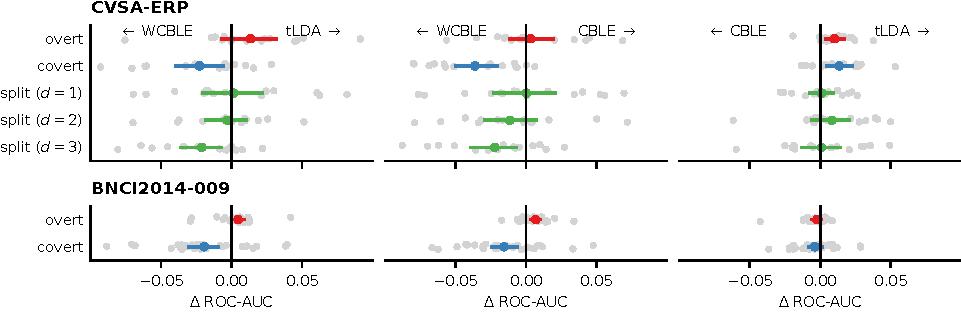
\includegraphics[width=\linewidth]{figures/covert_align/figure4a.pdf}
	\end{subfigure}

	\bigskip

	\begin{subfigure}{\linewidth}
		\caption{}
		\label{fig:covert-align/block-eval}%
		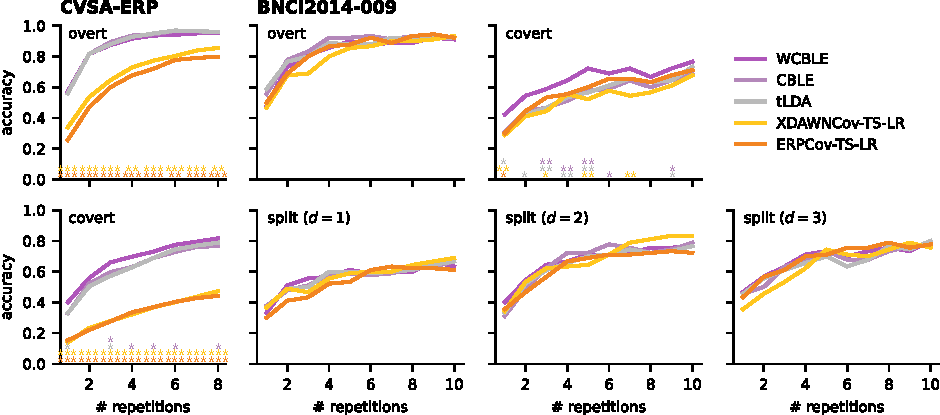
\includegraphics[width=\linewidth]{figures/covert_align/figure4b.pdf}
	\end{subfigure}
  \caption[Decoder performance.]{%
		\subref{fig:covert-align/single-trial-roc-auc-diff} Difference in cross-validated
    single-trial classification \acl{rocauc} ($\Delta$ROC-AUC)
    between \ac{cble}, \ac{wcble}, and their first-stage classifier \ac{tlda}.
    95\% confidence intervals were determined using $k=1000$ bootstrapping.
    Our proposed \ac{wcble} decoder outperforms \ac{tlda} and \ac{cble} for covert and split
    ($d=3$)	\ac{vsa}. \ac{cble} scores on par with \ac{tlda}.
		\subref{fig:covert-align/block-eval} Cross-validated target selection accuracy for
    all decoders plotted as a function of the number of test repetitions in
    different VSA conditions. Significance was determined using one-sided
    (\ac{wcble} $>$ other) Wilcoxon signed-rank tests using False Discovery Rate correction
    ($*= p<0.05$, $**=p<0.01$, $***=p<0.001$). \ac{wcble} generally achieves the highest
    covert \ac{vsa} target selection accuracy.}
\end{figure}

Wilcoxon signed-rank tests controlled for multiple comparisons by Benjamini
and Hochberg's False Discovery Rate procedure (FDR) revealed that
for the BNCI2014-009 dataset, \ac{wcble} significantly outperformed \ac{tlda}
($\Delta\mathrm{ROC-AUC} = 0.019$, $p=0.004$) and \ac{cble}
($\Delta\mathrm{ROC-AUC} = 0.016$, $p=0.036$) for covert \ac{vsa},
but was significantly outperformed by \ac{tlda} in overt \ac{vsa} decoding
($\Delta\mathrm{ROC-AUC}=-0.004$, $p=0.040$).
For the CVSA-ERP dataset, \ac{wcble}
also achieved significantly better covert \ac{vsa} performance than \ac{tlda} ($\Delta\mathrm{ROC-AUC}
	= 0.023$, $p=0.041$) and \ac{cble} ($\Delta\mathrm{ROC-AUC}
	= 0.036$, $p=0.024$).
We found no significant difference in \ac{wcble} performance over \ac{tlda} in the split
\ac{vsa} conditions in the CVSA-ERP dataset, but results show a clear trend of
increased \ac{wcble} performance over \ac{tlda} and \ac{cble} as $d$ increases.
\ac{cble} failed to significantly outperform its first-stage classifier \ac{tlda} in all
evaluated \ac{vsa} conditions.
\Cref{tab:covert-align/results/single-trial} reports all single-trial classification scores for all considered models, datasets, and conditions.

\Cref{fig:covert-align/block-eval} shows the cross-validated \ac{bci} selection
accuracy on the BNCI2014-009 and the CVSA-ERP datasets for all investigated
decoders.
Accuracy was determined by, for each block, selecting the character with the
highest (stage-two if applicable) classifier score and comparing it to the cued target.
Significance was calculated using one-sided Wilcoxon signed-rank tests ($p=0.05$)
corrected for FDR over decoders.
For this evaluation, no epochs were rejected to keep the trial-based structure
of \ac{bci} operation intact.
For all datasets and \ac{vsa} conditions, \ac{cble} scores approximately on par with \ac{tlda}.
Yet, \ac{wcble} yields an improved decoding accuracy for covert \ac{vsa} in both
datasets, which is greatest for smaller numbers of repetitions and
decreases as the number of repetitions increases.
This covert \ac{vsa} accuracy increase over \ac{tlda} is significant in the
BNCI2014-009 dataset for 1 and 3 repetitions, and in CVSA-ERP for 1-5 and 10 repetitions.
Furthermore, while we reported a relative decrease in single-trial \ac{rocauc} for
\ac{wcble} in overt \ac{vsa}, this does not seem to result in a consistent decrease in target
selection accuracy.
No significant increase of \ac{wcble} over other methods was found in split \ac{vsa}.
While Riemannian methods are significantly outperformed by \ac{tlda}, \ac{cble}, and \ac{wcble}
in the BNCI2014-009 dataset, they perform approximately on par with \ac{tlda} and
\ac{wcble} in CVSA-ERP.

Overall, we observed a 5.10\%pt. accuracy increase with \ac{wcble} over
\ac{tlda} for covert \ac{vsa} in the BNCI2014-009 dataset and 5.55\%pt. in the CVSA-ERP dataset.
These results compare to the performance gain reported by \textcite{Zisk2022}.
They observed a 5.63\%pt. accuracy increase with 1-10 selection repetitions over
step-wise Linear Discriminant Analysis  (SWLDA) for 6 participants with
\ac{als}, whose SWLDA performance also suffered from jitter.
Note that interpretation of this comparison may be challenging due to differences in
interface design (number of targets, \ac{isi}), subject population,
\ac{eeg} recording procedure, and available training data.

\subsection{Gaze-independence through cross-condition transfer}
\label{sec:covert-align/results/cross}
To further back our claim of gaze-independence in the case where eye motor
control cannot be assumed, we evaluate our proposed decoder in a transfer
learning setting between \ac{vsa} conditions.
While performing overt attention requires gaze redirection for each target
selection, performing covert or split \ac{vsa} continuously still requires
sustained gaze fixation, which might be impaired in those who
could benefit from such an application.
Studying the transfer between conditions simulates what happens
when the user performs different \ac{vsa} conditions throughout the
experimental session.
Furthermore, if our decoder performs well in transfer-learning settings,
it must capture some information about the \ac{erp} responses that is independent of
the \ac{vsa} condition, and hence does not depend on gaze redirection to perform
these conditions.
We introduce an additional setting of interest here, namely a combination of \ac{vsa}
conditions, which represents those cases where the user cannot
redirect their gaze and hence can be in any one of the \ac{vsa} conditions depending on the
target they attend to.
For BNCI2014-009, this is implemented as an equal mix of overt and
covert \ac{vsa}; for CVSA-ERP, the combined condition represents an equal mix of overt,
covert, and split \ac{vsa}, disregarding parameter $d$.

\Cref{fig:covert-align/covert-cross-eval} and \cref{fig:covert-align/aloise2012-cross-eval} show
the pairwise differences in area under the ROC curve ($\Delta$ROC-AUC)
between the investigated decoders.
In this evaluation, bad epochs were rejected as in \cref{sec:covert-align/results/bloc-acc}.
\begin{figure*}
  \bigskip
	\begin{subfigure}{\linewidth}
		\caption{}
		\label{fig:covert-align/covert-cross-eval}
		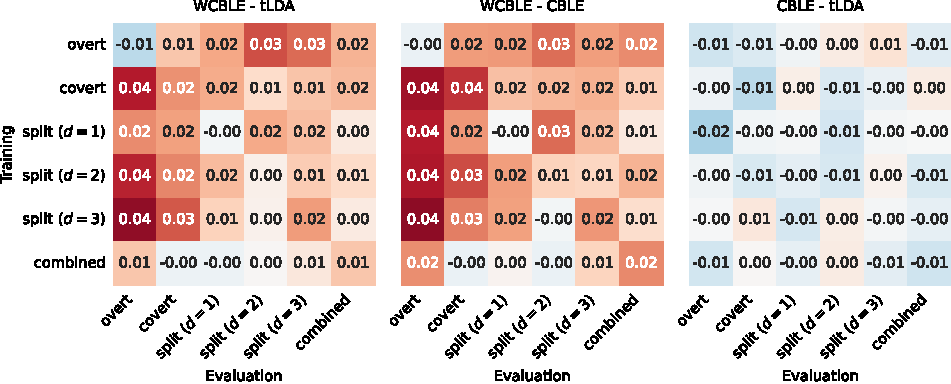
\includegraphics[width=\linewidth]{figures/covert_align/figure5a.pdf}
	\end{subfigure}

	\bigskip
	\bigskip

	\begin{subfigure}[c]{.48\linewidth}
		\caption{}
		\label{fig:covert-align/aloise2012-cross-eval}
		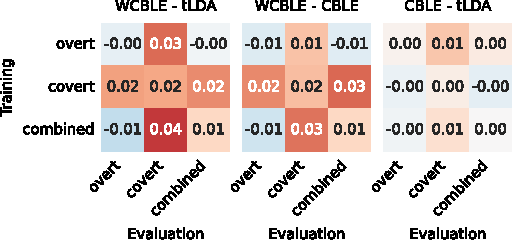
\includegraphics[width=\linewidth]{figures/covert_align/figure5b.pdf}
	\end{subfigure}\hfill%
	\begin{subfigure}[c]{.48\linewidth}
		\caption{}
		\label{fig:jitter}
		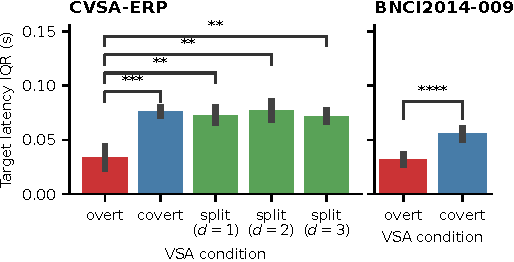
\includegraphics[width=\linewidth]{figures/covert_align/figure5c.pdf}
	\end{subfigure}

  \caption[Cross-condition classifier performance and estimated jitter.]{
		\subref{fig:covert-align/covert-cross-eval},\subref{fig:covert-align/aloise2012-cross-eval}
    Difference in cross-validated area under the receiver
		operating characteristic curves between Classifier-based Latency Estimation
    (CBLE) and Woody CBLE (WCBLE) across conditions for the CVSA-ERP and
    BNCI2014-009 datasets, respectively.
    A decoder is each	time trained on a visuospatial attention (VSA) condition
    and tested on all VSA conditions.
    WCBLE yields an improvement in most
		non-overt \ac{vsa} settings, indicating it is more invariant to eye gaze than
    CBLE and \ac{tlda}.
		\subref{fig:jitter} Jitter characterized as the interquartile range (IQR)
		of target epochs for different \ac{vsa} conditions. Overt \ac{vsa} exhibits lower
    jitter than other conditions.
    Significance of differences
    was determined with two-sided Wilcoxon signed-rank tests with False Discovery
    Rate correction on per-subject jitter ($*= p<0.05$, $**=p<0.01$,
    $***=p<0.001$, $****=p<0.0001$).
	}
\end{figure*}
When comparing \ac{cble} and \ac{tlda}, we do not observe large differences in any of the
evaluated settings, similar to the within-subject conditions, with the greatest
\ac{rocauc} difference -2\% for training in split $(d=2)$ \ac{vsa} and overt \ac{vsa}.
On the contrary, when considering the comparisons between \ac{wcble} and \ac{tlda}, we
see that performance is on par or greater using \ac{wcble} for most conditions,
except for within-overt \ac{vsa} decoding, with the greatest \ac{rocauc}
difference +4\% for training in split ($d=2$) \ac{vsa} and testing in overt
\ac{vsa}.


\subsection{Jitter analysis}
\label{sec:covert-align/results/jitter}
Finally, an analysis is performed to quantify the jitter presence in the
different \ac{vsa} conditions.
To obtain comparable results across \ac{vsa} conditions, \ac{wcble} was
evaluated per session and trained on all combined \ac{vsa} conditions as in
\cref{sec:covert-align/results/cross}.
Since all conditions have the P3 in common, the estimated latencies can be
interpreted as P3 latencies.
Results are shown in \cref{fig:jitter}.

Two-sided Wilcoxon rank-sum tests on jitter, expressed as the interquartile
range (IQR) of the estimated latencies of target trials, revealed that overt
\ac{vsa} exhibited significantly lower jitter than all other conditions for
both datasets, with jitter equal to overt: 32 ms and covert:
56 ms ($p<0.001$) for BNCI2014-009, and overt: 33 ms, covert: 77 ms ($p<0.001$),
split ($d=1$): 72 ms ($p=0.006$),
split ($d=2$): 77 ms ($p=0.002$)
and split ($d=3$): 72 ms ($p=0.002$)
for CVSA-ERP.
No other significant differences were found.
$p$-values were corrected for the family-wise error rate using Bonferroni
correction.

\section{Discussion}

\Cref{fig:covert-align/single-trial-roc-auc-diff} shows that \ac{wcble} significantly improves
covert \ac{vsa} decoding.
This is advantageous for the development of a class of \ac{erp}-\ac{bci} interfaces for
users who prefer to rest their gaze on a fixation cross on the screen,
avoiding the effort of redirecting their eye gaze for every selection.
Furthermore, the performance gain over the first-stage classifier in split
\ac{vsa} ($d=3$) and between-\ac{vsa} condition transfer settings are promising for
users with even less eye motor control who may experience involuntary eye
movements or fixation fatigue and hence cannot keep their gaze fixed throughout an
entire \ac{bci} operation session.
\ac{wcble} would allow them to operate a \ac{bci} comfortably while directing
their gaze to whichever portion of the screen they prefer, even when there is
another target present or this location varies during the
course of operation.
Although \ac{wcble} did not significantly improve overt \ac{vsa} single-trial decoding,
\cref{fig:covert-align/block-eval} shows that this does not negatively impact target
selection accuracy.
While target selection accuracy also did not improve for split \ac{vsa}, the
increase in single-trial performance in split ($d=3$) shows that an iterative
alignment procedure has the potential to improve over \ac{cble} and its first-stage
classifier in this case as well.


We believe the relative increase in performance of our proposed decoder in covert and
split \ac{vsa}, and the lack thereof in overt \ac{vsa}, could stem from the following:
\begin{enumerate*}[label=(\arabic*)]
  \item Covert and split \ac{vsa} exhibit higher P3 jitter than overt \ac{vsa}.
        In covert and split \ac{vsa}, participants have to execute a dual task by
        dissociating their visuospatial attention and gaze fixation.
        Evidence shows that \ac{erp} latency variability is
        higher when attention is divided~\cite{Polich2007,Arico2014}.
        \textcite{Arico2014} also partly attribute higher latency jitter to the covert \ac{vsa}
        task performed in the BNCI2014-009 dataset, since the GeoSpell interface
        requires both spatial and feature attention.
  \item In overt \ac{vsa}, the first-stage classifier can rely mostly on the modulation
        of early visually evoked potentials (VEPs) like N1 rather than on the
        P3~\cite{Treder2010}.
        These VEPs are closely related to visual processing, hence exhibit
        lower jitter, contrary to P3, which is more prone to the effects of
        attention and workload~\cite{Hu2010}, reducing the contribution of
        alignment.
  \item This property can also result in the estimation of VEP latencies
        instead of the P3 latency, and \ac{wcble} would in this case fail to
        increase the P3 \ac{snr}, which still could be somewhat jittered in overt
        \ac{vsa}.
  \item Aligning to the P3 will lower the \ac{snr} of early VEPs, while aligning to
        VEPs will lower P3 \ac{snr}, since they are not time-locked to each other.
	\item Covert and split \ac{vsa} \acp{erp} may exhibit lower \ac{snr} than overt
        \ac{vsa} due to lower P3 amplitudes or even due to the presence of higher P3
        jitter itself.
        Higher \ac{snr} in overt \ac{vsa} results in higher decoding performance of
        state-of-the-art classifiers, leaving less room for relative improvement
        in this case.
\end{enumerate*}

Although it is not immediately clear if \ac{wcble} actively corrects for higher P3 jitter
present in covert and split \ac{vsa} compared to overt \ac{vsa},
we justify our approach in a similar manner to \textcite{Hardiansyah2020} by
observing that the increased discrimination performance of a machine-learning
model accounting for jitter forgoes the need for characterizing the underlying
physiological processes, while still objectively quantifying the presence of
jitter between data classes.
Furthermore, some evidence points toward higher P3 jitter as the main
contributing factor.
While \autoref{fig:erps} shows no visible smearing effect in
the shape of the \acp{erp}, the more quantitative analysis on latencies
presented in \cref{sec:covert-align/results/jitter}
indicates the opposite.
Additionally, \textcite{Arico2014} prove that P3 jitter does play a
non-negligible role in covert \ac{vsa} by comparing performance between
overt and covert \ac{vsa}, while including or excluding early VEPs.
This analysis showed that the absence of the N1 and other early VEPs is not the
only factor hampering covert \ac{vsa} decoding performance.
However, the large increase in accuracy for covert \ac{vsa} reported by
\textcite{Arico2014} (60\% to 95\% with a window focusing on only the P3
component) could also be explained by overfitting on artifacts amplified by
aligning, since their method is not evaluated on unseen data, as opposed to ours.

We also argue that \ac{wcble} does not only enhance the P3 signal, but effectively reduces the
negative impact of noise that would otherwise mask the \ac{erp} response, thereby increasing the
discriminative ability of the decoder.
This process likely results in more reliable feature extraction, especially in conditions
with high jitter.

We found that \ac{cble} did not improve gaze-independent decoding performance
significantly and also did not increase performance over its first-stage
classifier in overt \ac{vsa}, contrary to what was reported by \textcite{Mowla2017}.
While they report that \ac{cble} is relatively independent of the
first-stage classifiers evaluated in their work, it is evident here that
applying any given classifier in the \ac{cble} scheme does not necessarily increase
its performance.
In our case, this could be due to characteristics of the tested dataset, e.g.,
the presence of jitter or the generally higher performance of \ac{tlda} compared to the
first-stage classifiers tested by \textcite{Mowla2017}, leaving less
performance to be gained.

\textcite{Thompson2012} already attempted applying \ac{cble} in an iterative scheme
but did not report any results due to convergence issues.
We mitigated this by combining the robust latency estimation presented in
\cref{sec:robust-latency} with the alignment of both target and non-target
epochs.
Aligning only the target epochs containing the jittered P3 component is prone to
overfitting by aligning non-discriminative noise that is present in both
classes, such as environment noise, oscillatory background rhythms, or
non-modulated VEPs.
If \ac{snr} is low, residual noise varying slightly between classes could dominate
the expected response of the first-stage classifier and subsequently dominate
\ac{wcble} from the start, preventing convergence to a meaningful solution.
Our procedure circumvents this problem by aligning both classes to the time
points where the expected separation between classes is greatest.
This way, noise of which the latencies are estimated in a given iteration will be
perfectly time-locked in all classes in the next
iteration.
The first-stage classifier can then more easily suppress this noise since it is
now clear it is present in both classes and non-discriminative.
This aids the method in converging to a more robust classifier by iteratively
increasing \ac{snr} for both classes and class separation over time.

\textcite{Zisk2022} addressed P3 jitter inparticipants \ac{als} by augmenting the
training data once with time-shifted copies based on \ac{cble}-estimated jitter.
While we aim to train the first-stage classifier without the effects of jitter
in its parameters, they do the opposite by intentionally jittering the
training data.
As their focus was on \ac{als} and inter-session stability, they
did not assess how their method interacts with visuospatial attention.
We achieved a similar performance gain with our jitter compensation method, but
argue that our method can cope with more granular latency differences, as
\textcite{Zisk2022} augment the data with just one positive and negative time
shift.

\textcite{Hardiansyah2020} decoded covert \ac{vsa} more effectively by
contributing single-trial latency and amplitude features for decoding.
Contrary to our approach, they did not correct these amplitude
features for the jitter in their latencies by, e.g., aligning trials to achieve
better separability.
Hence, their approach would not, in principle, render the classifier more robust
to jitter.
Furthermore, we incorporated estimated latency features in both \ac{cble} and \ac{wcble},
yet only \ac{wcble} improved covert \ac{vsa} performance.
This shows that the incorporation of latency features is not the only driver of
covert \ac{vsa} decoding performance increase.

Despite encouraging results, our study faces some limitations that we plan to
tackle in the future.
Firstly, multiple \ac{erp} components can be time-locked to different neural
processes, each with its own jitter, hampering the performance of
single-trial latency estimation and their interpretability.
Adaptations could be made to incorporate prior time windows or probability
distributions on the latency of specific \ac{erp} components or to simultaneously
estimate a set of multiple component (clusters) latencies per \ac{erp}, such as in Residue Iteration
Decomposition~\cite{Ouyang2017}.
Future efforts should investigate how strong
spatiotemporal filtering can be combined with methods that allow for a more
flexible non-stationarity of the \ac{erp}, like Dynamic Time Warping (DTW) or other
techniques borrowed from time series classification, or methods that explicitly model multiple time
displacements present in one \ac{erp}.


Secondly, performance might be improved by venturing beyond the classical
target/non-target binary classification problem.
Due to, for example, the perifoveal stimulus cruciform model~\cite{Vanegas2013}, covert and split \ac{vsa}
responses might differ based on the relative position in the field of view of
their related stimulus, which could be exploited in a multi-class classification
problem.
Similarly, explicitly taking into account the characteristics of the distractor \ac{erp}
response might have a beneficial effect.
Thirdly, results were obtained in an offline and within-session evaluation,
which does not reflect true \ac{bci} operation.
Using multiple sessions with online feedback, the user could optimize their
performance over time by controlling attention or gaze.
Finally, since this work was conducted with applications for individuals with
\ac{sspgi} in mind, we
should highlight that the gaze of participants in the conducted experiments was
cued and fixed, which is per definition impossible for the end user group we consider.
In \cref{sec:patients}, we present a study to further investigate whether the
studied \ac{vsa} conditions are appropriate and to what extent they occur when
individuals with \ac{sspgi} operate a \ac{bci}.

\section{Conclusion}

Our aim was to improve gaze-independent \ac{bci} performance for spatially
organized visual event-related potential (\ac{erp}) paradigms by using a suitable
decoder.
Earlier results on \ac{bci} performance in covert visuospatial attention
(\ac{vsa}) performance prediction have shown that accounting for single-trial
latency jitter could improve gaze-independent decoding performance.
We applied Classifier-based Latency Estimation (\ac{cble}) as a decoder robust to latency
jitter, but found no increase in gaze-independent decoding performance.
To remedy this, we improved \ac{cble} by adapting it into \ac{cble} with Woody
iterations (\ac{wcble}), an iterative scheme using probabilistic latency estimation.
Results for \ac{wcble} within and across \ac{vsa} condition decoding show that
gaze-independent \ac{bci} performance can be improved at the decoding stage.
Overt decoding performance was not improved, but our proposed method can
provide added value for users who are unable to operate a visual \ac{bci} in overt
attention mode.
Later studies should confirm whether our findings hold in individuals with
severe physical impairment and a variety of eye-motor impairments, and develop a
solution that is capable of properly handling multiple non-time-locked \ac{erp}
components.

\clearpage
\begin{subappendices}
  \section{Single-trial classification performances}
  \begin{table}[ht]
  \centering
  \makebox[\textwidth][c]{%
    \begin{tabular}{lccccccc}
\toprule
dataset & \multicolumn{2}{c}{BNCI2014-009} & \multicolumn{5}{c}{CVSA-ERP} \\
\cmidrule(lr){2-3} \cmidrule(lr){4-8}
VSA condition & overt & covert & overt & covert & split ($d=1$) & split ($d=2$) & split ($d=3$) \\
\midrule
ERPCov-TS-LR    & 0.9000     & 0.7450        & 0.7956     & 0.6880      & 0.6690      & 0.7252      & 0.7214 \\
XDAWNCov-TS-LR  & 0.9044     & 0.7464        & 0.8113     & 0.6780      & 0.6683      & 0.7259      & 0.7136 \\
tLDA            & 0.9474     & 0.7890        & 0.\bf 8660 & 0.7111      & \bf 0.7097      & 0.7550      & 0.7474 \\
CBLE            & \bf 0.9497 & 0.7928        & 0.8559     & 0.6977      & 0.7087  & 0.7467      & 0.7465 \\
WCBLE           & 0.9428     & \bf 0.8084    & 0.8525     & \bf 0.7338  & 0.7084      & \bf 0.7581  & \bf 0.7687 \\
\bottomrule
\end{tabular}

  }
  \caption{Cross-validated single-trial classification area under the receiver operating characteristic
curve for all evaluated models, visuospatial attention conditions, and
  datasets.}
  \label{tab:covert-align/results/single-trial}
\end{table}

  \clearpage
  \section{Cross-condition transfer classification performances}

  \begin{table}[ht]
      \footnotesize
      \sffamily
\small
\begin{tabularx}{\textwidth}{@{}XXrrrrrr@{}}
\toprule
  & test & overt & covert & \makecell[r]{split \\ ($d=1$)} & \makecell[r]{split
  \\($d=2$)} & \makecell[r]{split \\ ($d=3$)} & combined \\
classifier & train &  &  &  &  &  &  \\
\midrule
\multirow[t]{6}{*}{CBLE} & overt & 85.59 & 66.68 & 63.92 & 60.22 & 60.11 & 66.25 \\
 & covert & 68.51 & 69.77 & 70.52 & 68.50 & 70.29 & 75.08 \\
 & split ($d=1$) & 64.11 & 67.81 & 70.87 & 69.60 & 69.44 & 75.04 \\
 & split ($d=2$) & 60.48 & 67.59 & 69.99 & 74.67 & 72.88 & 75.96 \\
 & split ($d=3$) & 59.32 & 69.66 & 68.51 & 72.95 & 74.65 & 75.18 \\
 & combined & 68.77 & 73.71 & 74.36 & 76.41 & 75.14 & 72.73 \\
\midrule
\multirow[t]{6}{*}{tLDA} & overt & 86.60 & 67.40 & 64.15 & 59.80 & 59.39 & 66.85 \\
 & covert & 68.78 & 71.11 & 70.17 & 69.25 & 70.64 & 74.69 \\
 & split ($d=1$) & 65.72 & 68.00 & 70.97 & 70.53 & 69.52 & 75.07 \\
 & split ($d=2$) & 60.69 & 68.40 & 70.48 & 75.50 & 72.69 & 76.75 \\
 & split ($d=3$) & 59.37 & 69.10 & 69.40 & 72.56 & 74.74 & 75.61 \\
 & combined & 69.71 & 73.64 & 74.81 & 76.01 & 75.68 & 73.78 \\
\midrule
\multirow[t]{6}{*}{WCBLE} & overt & 85.25 & 68.80 & 66.07 & 63.02 & 62.22 & 68.60 \\
 & covert & 72.75 & 73.38 & 72.02 & 70.16 & 72.06 & 76.30 \\
 & split ($d=1$) & 68.07 & 70.04 & 70.84 & 72.42 & 71.05 & 75.56 \\
 & split ($d=2$) & 64.53 & 70.84 & 72.07 & 75.81 & 73.97 & 77.70 \\
 & split ($d=3$) & 63.79 & 72.21 & 70.57 & 72.80 & 76.87 & 76.05 \\
 & combined & 71.09 & 73.36 & 74.53 & 76.07 & 76.26 & 75.15 \\
\bottomrule
\end{tabularx}

      \caption[Transfer learning results for CVSA-ERP]{Cross-condition transfer
      classification performance (cross-validated \ac{rocauc})
      for all evaluated models in the CVSA-ERP dataset. Each decoder is trained
      on one \ac{vsa} condition and tested across all
      \ac{vsa}
      conditions to evaluate gaze-independence and transfer learning
      performance.}
  \end{table}
  \begin{table}[ht]
      \footnotesize
      \sffamily
\small
\begin{tabular}{@{}llrrr@{}}
\toprule
 & test & overt & covert & combined \\
classifier & train &  &  &  \\
\midrule
\multirow[t]{3}{*}{CBLE} & overt & 94.97 & 63.59 & 83.13 \\
 & covert & 67.00 & 79.28 & 73.01 \\
 & combined & 93.81 & 73.36 & 83.17 \\
\midrule
\multirow[t]{3}{*}{tLDA} & overt & 94.74 & 62.22 & 82.70 \\
 & covert & 67.34 & 78.90 & 73.51 \\
 & combined & 94.01 & 72.55 & 83.16 \\
 \midrule
\multirow[t]{3}{*}{WCBLE} & overt & 94.28 & 65.04 & 82.51 \\
 & covert & 69.40 & 80.84 & 75.87 \\
 & combined & 92.77 & 76.10 & 84.20 \\
\bottomrule
\end{tabular}

      \caption[Transfer learning results for BNCI2014-009]{Cross-condition transfer
      classification performance (cross-validated \ac{rocauc})
      for all evaluated models in the CVSA-ERP dataset. Each decoder is trained
      on one \ac{vsa} condition and tested across all \ac{vsa}
      conditions to evaluate gaze-independence and transfer learning
      performance.}
  \end{table}
\end{subappendices}
